\documentclass[a4paper]{article}

\usepackage[utf8]{inputenc}
\usepackage[T1]{fontenc}
\usepackage{textcomp}
\usepackage[italian]{babel}
\usepackage{amsmath, amssymb}
\usepackage{amsfonts}
\usepackage{mdframed}
\usepackage{ntheorem}
\usepackage{xcolor}
\usepackage{float}
\usepackage{graphicx}
\graphicspath{{./figures/}}

\usepackage{import}
\usepackage{pdfpages}
\usepackage{transparent}
\usepackage{xcolor}

% Useful definitions frame
\theoremstyle{break}
\theoremheaderfont{\bfseries}
\newmdtheoremenv[%
linecolor=gray,leftmargin=0,%
rightmargin=0,
innertopmargin=8pt,%
ntheorem]{define}{Definizioni utili}[section]

% Example frame
\theoremstyle{break}
\theoremheaderfont{\bfseries}
\newmdtheoremenv[%
linecolor=gray,leftmargin=0,%
rightmargin=0,
innertopmargin=8pt,%
ntheorem]{example}{Esempio}[section]

% Important definition frame
\theoremstyle{break}
\theoremheaderfont{\bfseries}
\newmdtheoremenv[%
linecolor=gray,leftmargin=0,%
rightmargin=0,
backgroundcolor=gray!40,%
innertopmargin=8pt,%
ntheorem]{definition}{Definizione}[section]

% Exercise frame
\theoremstyle{break}
\theoremheaderfont{\bfseries}
\newmdtheoremenv[%
linecolor=gray,leftmargin=0,%
rightmargin=0,
innertopmargin=8pt,%
ntheorem]{exercise}{Esercizio}[section]


% figure support
\usepackage{import}
\usepackage{xifthen}
\pdfminorversion=7
\usepackage{pdfpages}
\usepackage{transparent}
\newcommand{\incfig}[1]{%
  \def\svgwidth{\columnwidth}
  \import{./figures/}{#1.pdf_tex}
}

\pdfsuppresswarningpagegroup=1

\begin{document}
\section{Cinematica}
\subsection{Moto in una dimensione}
\[
  \text{Velocità: } \vec{v} = \frac{\Delta \vec{r}}{\Delta t}
\] 
\[
  \text{Accelerazione: } \vec{a} = \frac{\Delta \vec{v}}{\Delta t}
\] 
\subsubsection{Moto rettilineo uniforme}
\[
x(t) = x_i + v_i t
\] 

\subsubsection{Moto rettilineo uniformemente accelerato}
\[
  x(t) = x_i + v_i t + \frac{1}{2} a t^2
\]
\[
  v(t) = v_i + a t
\]
\[
  v^2 = v_i^2 + 2 a \cdot \Delta x
\]
\[
  t = \frac{v_f - v_i}{a}
\] 

\subsection{Moto in due dimensioni}
\subsubsection{Moto parabolico}
\[
  x = x_i + v_{ix} t
\] 
\[
  y = y_i + v_{iy} t - \frac{1}{2} g t^2
\]
\vspace{1em}
\[
  v_x = v_{ix}
\]
\[
  v_y = v_{iy} - g t
\]

\vspace{1em}
\[
  h_{max} = \frac{v_i^2 \sin^2 \theta}{2g}
\] 
\[
  R_{gittata} = \frac{v_i^2 \sin 2\theta}{g}
\] 
\textbf{Informazioni sull'altezza massima:}

\noindent Nel punto di altezza massima di un moto parabolico, la velocità verticale vale
sempre \( 0 \), e la distanza orizzontale percorsa vale metà della gittata. (più un eventuale
\( x_0 \)  iniziale)

\subsection{Moto circolare}
\[
  \text{Spostamento angolare: } \Delta \varphi
\] 
\[
  \text{Velocità angolare: } \omega = \frac{\Delta \varphi}{t} = \frac{2 \pi}{T}
\]
\[
v = r \omega
\] 
\[
  \text{Accelerazione angolare: } \alpha = \frac{\Delta \omega}{t}
\] 
\begin{itemize}
  \item Moto circolare uniforme: 
    \[
      \varphi = \varphi_i + \omega_i t
    \] 
    \[
      \omega = \omega_i
    \]
    \[
      t = \frac{\varphi_f - \varphi_i}{\omega}
    \]
  \item Moto circolare uniformemente accelerato:
    \[
      \varphi = \varphi_i + \omega_i t + \frac{1}{2} \alpha t^2
    \]
    \[
      \omega = \omega_i + \alpha t
    \]
    \[
      \omega^2 = \omega_i^2 + 2 \alpha \Delta \varphi
    \]
    \[
      t = \frac{\omega_f - \omega_i}{\alpha}
    \]
\end{itemize}
\vspace{1em}
\[
  F_{centripeta} = m r \omega^2
\] 

\noindent \textbf{Informazioni utili:}

\noindent Nel moto circolare esiste una accelerazione centripeta che segue la direzione 
del raggio che collega il corpo al centro della circonferenza, e si occupa di mantenere 
l’oggetto nella traiettoria. Se il moto è solo circolare uniforme non vi è accelerazione 
tangenziale. 
\[
  a_{centr} = \frac{v^2}{r} = r \omega^2
\] 

\vspace{1em}
\noindent Se il moto è circolare uniformemente accelerato oltre all’accelerazione 
centripeta vi sarà anche quella tangenziale, dunque l’accelerazione totale sarà la somma
vettoriale. (\( \vec{a}_{centr} + \vec{a}_{tang} = \vec{a}_{tot} \) ) 

\[
  a_{tang} = r \alpha
\]  

\vspace{1em}
\noindent In un moto circolare, la forza d’attrito statico (se presente) funge 
da forza centripeta.


\section{Moto armonico}
\[
\begin{cases}
  x(t) = A \cos(\omega t + \varphi)\\
  v(t) = -A \omega \sin(\omega t + \varphi)\\
  a(t) = -A \omega^2 \cos(\omega t + \varphi)
\end{cases}
\] 
L'accelerazione è la tendenza a tornare al punto di equilibrio.
\[
\omega = \frac{2 \pi}{T} = 2 \pi \cdot f
\] 
\subsection{Molla}
\[
  \omega = \sqrt{\frac{k}{m}}
\] 
\( k \) è la costante elastica, \( m \) è la massa del corpo. 

\subsection{Pendolo}
\[
  \omega = \sqrt{\frac{g}{l}}
\]
\( l \) è la lunghezza del pendolo.

\section{Leggi del moto}
\subsection{Leggi di Newton}
\subsubsection{Prima legge di Newton}
Se la forza risultante che agisce su un sistema è nulla, vuol dire che il sistema o è in quiete o si muove
di moto rettilineo uniforme. (velocità costante)

\subsubsection{Seconda legge di Newton}
In un sistema di riferimento inerziale, l’accelerazione di un corpo è direttamente proporzionale alla
forza risultante, e inversamente proporzionale alla massa. (\( \vec{F}_{ris} = m \cdot \vec{a}_{corpo} \) )
\[
F = m a
\] 
\[
  F_{\perp} = F \cos \theta \quad F_{\parallel} = F \sin \theta
\] 

\[
  \sum F = m a_c = m \frac{v^2}{r}
\] 

\subsubsection{Terza legge di Newton}
Se due corpi interagiscono tra di loro, la forza \( F_{1 \to 2} \) esercitata dal corpo 1 sul corpo 2 è di uguale
intensità e verso opposto alla forza \( F_{2 \to 1} \) esercitata dal corpo 2 sul corpo 1.
(\( \vec{F}_{1 \to 2} + \vec{F}_{2 \to 1} = 0 \) )


\section{Forze, lavoro ed energia}
\subsection{Forze fondamentali}
\subsubsection{Forza peso}
\[
  \vec{F}_p = mg
\]
\subsubsection{Forza elastica}
\[
  \vec{F}_e = -k \Delta x
\]
\( -k \) è la costante elastica, \( \Delta x \) è la deformazione.
\subsubsection{Forza di attrito}
\begin{itemize}
  \item Attrito statico: \( F_{attrito} \leq \mu_s N \)
  \item Attrito dinamico: \( F_{attrito} = \mu_d N \)
\end{itemize}
\( N \) è la forza normale, \( \mu_s \) è il coefficiente di attrito statico, \( \mu_d \) è il coefficiente di attrito dinamico. 

\subsubsection{Forza di gravità}
\[
  \vec{F}_g = \frac{G m_1 m_2}{r^2} \hat{r}
\]
\( r \) è la distanza tra i due corpi, \( G \) è la costante di gravitazione universale (\( 6.67 \times 10^{-11} \, \text{N m}^2 / \text{kg}^2 \) )
e \( \hat{r} \) è il vettore unitario che collega i due corpi.

\subsection{Lavoro}
\subsubsection{Forza costante}
\[
  L = F \cdot d \cdot \cos \theta
\] 
\( d \) è lo spostamento e \( \theta \) l'angolo tra la forza e lo spostamento. 

\subsubsection{Forza elastica}
\[
  L = \frac{1}{2} k x^2
\]

\subsubsection{Forza peso}
\[
L = mgh
\] 
\( h \) è la variazione di altezza.

\subsection{Energia}
\subsubsection{Energia cinetica}
\[
  E_{cin} = \frac{1}{2} m v^2
\] 
\[
  L_{tot} = \Delta E_{cin}
\] 
\[
  \text{Potenza: } P = \frac{L}{\Delta t}\; [W]
\] 
Con forza e velocità costanti:
\[
P = F \cdot v
\] 

\subsubsection{Energia potenziale}
\[
  L_{cons} = - \Delta U
\] 
\[
  U_{peso} = mgh
\]

\subsubsection{Energia meccanica}
\[
  E_{mecc} = E_{cin} + U
\]
\[
  L_{non-cons} = \Delta E_{mecc} = \Delta E_{cin} + \Delta U
\] 

\section{Quantità di moto e urti}
\subsection{Quantità di moto}
\[
  \vec{p} = m \vec{v}
\]
\subsection{Impulso}
\[
  \vec{I} = \vec{p}_f - \vec{p}_i = \Delta \vec{p} = \vec{F} \Delta t
\]
\textbf{Teorema dell'impulso:}

\noindent L’impulso esercitato su un oggetto è uguale alla variazione di quantità di moto generata, che a sua
volta è uguale alla forza esercitata per accelerare (o decelerare) il corpo moltiplicata per il tempo di
applicazione di tale forza sul corpo.

\subsubsection{Momento angolare}
\[
  \vec{L} = \vec{r} \times \vec{p}
\]
Intorno ad un asse fisso:
\[
  \vec{L} = I_{asse} \vec{\omega}
\]
\[
\text{Momento di inerzia: } I = \sum m_i r_i^2
\] 

\subsection{Conservazione di quantità di moto}
Se il sistema di corpi è isolato, cioè non subisce forze esterne:
\[
  \Delta \vec{p}_{tot} = 0
\]

\subsection{Urti}
\subsubsection{Urti elastici}
\[
  \Delta E_{c_{tot}} = 0 \quad \Delta \vec{p}_{tot} = 0
\] 
\[
  m_1 \left( v_{1i}^2 - v_{1f}^2 \right) = m_2 \left( v_{2f}^2 - v_{2i}^2 \right)
\] 
\[
  v_{1f} = \frac{m_1 - m_2}{m_1 + m_2} v_{1i} + \frac{2 m_2}{m_1 + m_2} v_{2i}
\] 
\[
  v_{2f} = \frac{2 m_1}{m_1 + m_2} v_{1i} + \frac{m_2 - m_1}{m_1 + m_2} v_{2i}
\] 
\subsubsection{Urti anelastici}
\[
  \Delta E_{c_{tot}} \neq 0 \quad \Delta \vec{p}_{tot} = 0
\]
Se i corpi si attaccano:
\[
  m_1 \vec{v}_{1i} + m_2 \vec{v}_{2i} = (m_1 + m_2) \vec{v}_f
\] 

\section{Sistemi a più corpi}
\subsection{Centro di massa}
\[
  x_{cm} = \frac{\sum m_i x_i}{\sum m_i}
\]
\[
  y_{cm} = \frac{\sum m_i y_i}{\sum m_i}
\]
\vspace{1em}
\[
  \vec{r}_{cm} = \frac{\sum m_i \vec{r}_i}{\sum m_i}
\] 
\( r \) è la posizione rispetto all'origine. 
\[
  \vec{v}_{cm} = \frac{\sum m_i \vec{v}_i}{\sum m_i}
\] 
\[
  \vec{a}_{cm} = \frac{\sum m_i \vec{a}_i}{\sum m_i}
\]
\subsubsection{Momento di inerzia}
\[
  I_{cm} = \sum m_i r_i^2
\]

\section{Rotazione corpo rigido attorno ad un asse fisso}
\subsection{Momenti della forza e inerzia}
\[
  \vec{\tau} = \vec{r} \times \vec{F}
\]
\[
  \sum \vec{\tau} = I \vec{\alpha}
\] 
Il momento di inerzia dipende dal corpo:

\noindent Per un punto materiale: \( I = m r^2 \)
\begin{figure}[H]
  \centering
  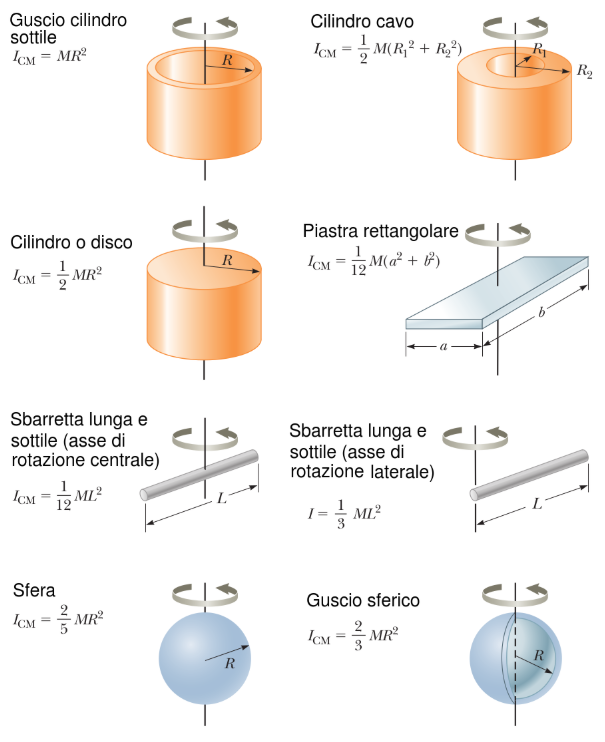
\includegraphics[width=0.8\textwidth]{inerzia}
  \caption{Momenti di inerzia notevoli}
  \label{fig:momenti_inerzia}
\end{figure}

\noindent \textbf{Informazioni sul momento: }
\noindent Il momento di una forza misura la capacità di una forza di mettere in rotazione un corpo intorno ad
un asse fisso. Il momento si calcola con il prodotto vettoriale tra \( \vec{r} \times \vec{F} \),,
ciò vuol dire che conta solo la componente perpendicolare della forza sul raggio.

\vspace{1em}
\noindent Per convenzione se \( \sum \tau > 0 \) si ha una rotazione antioraria del corpo
se \( \sum \tau < 0 \) invece si ha una
rotazione oraria, mentre se \( \sum \tau = 0 \) il corpo non ruota.

\vspace{1em}
\noindent Per la condizione di equilibrio statico, la somma dei momenti deve fare 0, non solo la somma delle
forze. Siccome si sta valutando una condizione d’equilibrio, posso permettermi di scegliere il perno
di rotazione ovunque io voglia, imponendo ogni volta che \( \sum \tau = 0 \).

\subsection{Energia e lavoro}
\[
  K_{rot} = \frac{1}{2} I \omega^2
\] 
\[
  L = \frac{1}{2} \omega_f^2 - \frac{1}{2} \omega_i^2
\] 

\subsection{Momento angolare}
\[
  L_{tot} = \left( \sum_i m_i r_i^2 \right) \omega = I \omega \quad \sum \tau_{est} = I \alpha
\] 

\textbf{Principio di conservazione del momento angolare:}
\noindent Se il momento dato dalle forze esterne al sistema è nullo, allora il momento angolare del sistema si
conserva.
\[
L_i = L_f \quad \iff \quad m_i \cdot r_i \cdot v_i = m_f \cdot r_f \cdot v_f \quad \iff \quad \omega_i \cdot I_i = \omega_f \cdot I_f
\] 

\section{Gravitazione}
\subsection{Prima legge di Keplero}
Tutti i pianeti percorrono orbite ellittiche, ed il Sole rappresenta uno dei due fuochi

\subsection{Seconda legge di Keplero}
Il raggio vettore passante per l’asse Sole-Pianeta spazza aree uguali in tempi uguali.

\subsection{Terza legge di Keplero}
Il quadrato del periodo di rivoluzione di un pianeta attorno al Sole è direttamente proporzionale al
cubo del semiasse maggiore dell’orbita.
\[
T^2 = k \cdot A^3
\] 
dove \( k \) è una costante del sistema solare e \( A \) è il semiasse maggiore dell’orbita.

\subsection{Legge di gravitazione universale}
Per la terza legge di Newton, due corpi esercitano sull’altro una forza
gravitazionale di uguale intensità con direzioni opposte.
\[
  F_{12} = -F_{21} = G \frac{m_1 m_2}{d^2}
\] 
dove \( G \) è la costante di gravitazione universale, \( m_1 \) e \( m_2 \) sono le masse dei corpi e \( d \) è la distanza tra i due corpi.

\subsection{Energia potenziale gravitazionale}
\[
  U_g = -G \frac{m_1 m_2}{d}
\] 

\subsection{Velocità di fuga}
Tramite l’energia potenziale gravitazionale è possibile calcolare quella velocità
per cui si può sfuggire al campo gravitazionale di un pianeta, dunque ogni
corpo celeste possiede la sua caratteristica velocità di fuga. (\( v_{f_{terra}} = 11.2 \frac{km}{s} \) )
\[
  v_{fuga} = \sqrt{\frac{2 G M}{r}}
\] 
dove \( M \) è la massa del pianeta e \( r \) è il raggio del pianeta.

\section{Termodinamica}
\subsection{Principi}
\subsubsection{Principio 0}
Se due sistemi termici sono separatamente in equilibrio termico con un terzo sistema, allora i primi
due sistemi sono in equilibrio termico tra di loro. Questa definizione apre al concetto di equilibrio
termico e temperatura di un corpo, stabilita tramite confronto con più corpi e determinando dei
valori di riferimento. Due corpi in equilibrio termico non presentano flussi di calore tra di loro.

\subsubsection{Primo principio}
L’energia totale di un sistema termodinamico (energia interna + lavoro scambiato con l’esterno) è
conservata sempre. La formula che rappresenta ciò è:
\[
  \Delta U_{sistema} = Q_{assorbito} - L_{compiuto}
\] 

\[
\text{Calore e capacità termica: } Q = C \cdot \Delta T
\] 
dove \( C \) è la capacità termica del corpo e \( \Delta T \) è la variazione di temperatura.

\[
  \text{Calore latente: } L_{t} = \frac{Q}{m}
\] 
Il calore latente di trasferimento è la quantità di calore necessaria per far
variare di una unità di massa la temperatura di un corpo.

\[
  \text{Entropia: } \Delta S_{AB} = \int_A^B \frac{dQ_{REV}}{T}
\] 
dove \( T \) è la temperatura e \( dQ_{REV} \) è il calore scambiato in maniera reversibile.

\subsubsection{Secondo principio}
È impossibile che un sistema operi in un ciclo termodinamico e converta completamente il calore
assorbito da una sorgente termica in lavoro meccanico senza produrre alcuna altra forma di effetto
o scambio di calore con l'ambiente circostante.

\subsection{Legge di stato dei gas}
La legge di stato dei gas impone che pressione e volume di un gas “ideale” siano inversamente
proporzionali tra di loro e proporzionali alla temperatura del corpo. Nella formula “n” rappresenta il
numero di moli e “R” la costante universale dei gas. La formula ha una controparte equivalente.
\[
  PV = nRT
\]
dove \( P \) è la pressione, \( V \) è il volume, \( n \) è il numero di moli, \( R \) è la costante universale dei gas e \( T \) è la temperatura.
\[
  R = 8.31 \frac{J}{mol \cdot K}
\] 
\[
PV = Nk_bT
\] 
dove \( N \) è il numero di particelle, \( k_b \) è la costante di Boltzmann.
\[
  k_b = 1.38 \times 10^{-23} \frac{J}{K}
\] 

\subsection{Equivalenze tra misure di pressione}
\[
1 \frac{N}{m^2} = 1\; \text{Pa} \quad 1\; \text{atm} = 1,013 \times 10^5\; \text{Pa} \quad
1 \;\text{bar} = 105 \;\text{Pa} \quad 1 \;\text{atm} = 760 \;\text{mmHg}
\] 

\subsection{Calore specifico}
\[
  \text{Per unità di massa: }  c = \frac{C}{m}
\] 
\[
  \text{Per mole: } c_{mol} = \frac{C}{n}
\] 
\[
\text{Per i solidi: } c = 3R
\] 
dove \( R \) è la costante universale dei gas.
\[
\text{Per i gas perfetti: } c_p - c_v = R
\] 
\begin{table}[H]
  \centering
  \begin{tabular}{r|c|c|c}
    & \( c_v \) & \( c_p \) & \( \gamma = \frac{c_p}{c_v} \) \\[0.2cm]
    \hline
    Monatomici & \( \frac{3}{2} R \) & \( \frac{5}{2} R \) & \(\frac{5}{3}\) \\[0.2cm]
    Biatomici & \( \frac{5}{2} R \) & \( \frac{7}{2} R \) & \(\frac{7}{5}\) \\
  \end{tabular}
\end{table}

\subsection{Gas perfetti}
\subsubsection{Energia interna}
\[
\Delta U = n c_v \Delta T
\] 

\subsubsection{Entropia}
\[
\Delta S = n c_v \ln \left( \frac{T_f}{T_i} \right) + n R \ln \left( \frac{V_f}{V_i} \right)
\] 

\subsubsection{Pressione di un gas in un tubo verticale}
\[
P = P_0 + \rho g h
\] 

\subsection{Trasformazioni termodinamiche}
\subsubsection{Isocora (\( \Delta V = 0 \))}
\[
L = 0 \quad Q = n c_v \Delta T
\] 
\begin{figure}[H]
  \begin{center}
    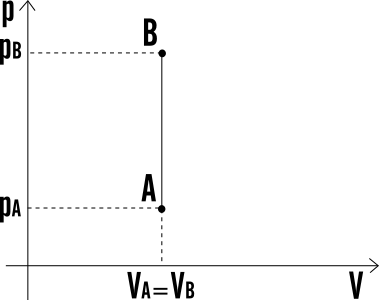
\includegraphics[width=0.4\textwidth]{isocora}
  \end{center}
  \caption{Grafico di una trasformazione isocora}
\end{figure}


\subsubsection{Isobara (\( \Delta P = 0 \))}
\[
L = -P \Delta V \quad Q = n c_p \Delta T
\] 
\begin{figure}[H]
  \begin{center}
    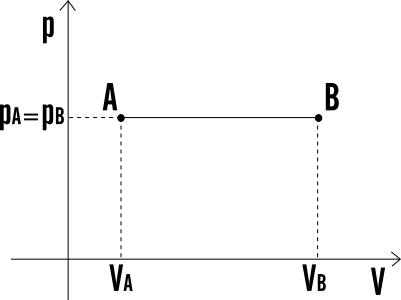
\includegraphics[width=0.4\textwidth]{isobara}
  \end{center}
  \caption{Grafico di una trasformazione isobara}
\end{figure}

\subsubsection{Isoterma (\( \Delta T = 0 \))}
\[
L = -Q \quad Q = n R T \ln \left( \frac{V_f}{V_i} \right)
\] 
\begin{figure}[H]
  \begin{center}
    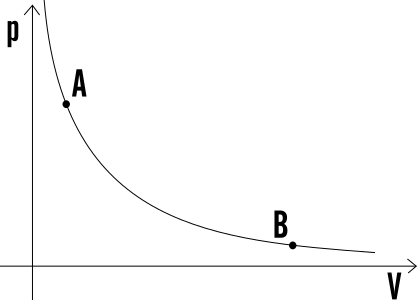
\includegraphics[width=0.4\textwidth]{isoterma}
  \end{center}
  \caption{Grafico di una trasformazione isoterma}
\end{figure}

\subsubsection{Adiabatica (\( Q = 0 \))}
\[
P V^\gamma = \text{costante}
\] 
\[
T V^{\gamma - 1} = \text{costante}
\] 
\[
  P^{1 - \gamma} T^\gamma = \text{costante}
\] 
dove \( \gamma = \frac{c_p}{c_v} \)
\[
L = \Delta U = \frac{1}{\gamma - 1} \left( P_f V_f - P_i V_i \right) 
\] 
\begin{figure}[H]
  \begin{center}
    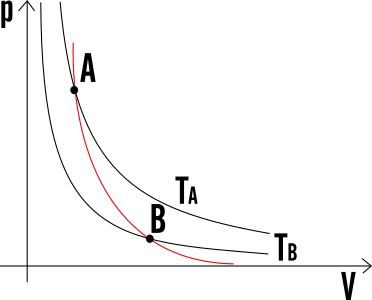
\includegraphics[width=0.4\textwidth]{adiabatica}
  \end{center}
  \caption{Grafico di una trasformazione adiabatica}
\end{figure}

\subsection{Macchine termiche}
\[
  \text{Efficienza: } \eta = \frac{L}{Q_{assorbito}} = 1 - \frac{Q_{ceduto}}{Q_{assorbito}}
\]
\[
\text{C.O.P. frigorifero: } \text{COP} = \frac{Q_{ceduto}}{L}
\] 
\[
  \text{C.O.P. pompa di calore: } \text{COP} = \frac{Q_{assorbito}}{L}
\] 
\[
\text{Efficienza di Carnot: } \eta = 1 - \frac{T_{ceduta}}{T_{assorbita}}
\] 
\[
  \text{Teorema di Carnot: } \eta < \eta_{reversibile}
\] 
\subsection{Espansione termica dei solidi}
\[
\text{Espansione lineare: } \frac{\Delta L}{L_i} = \alpha \Delta T
\] 
\[
\text{Espansione superficiale: } \frac{\Delta A}{A_i} = 2 \alpha \Delta T
\] 
\[
\text{Espansione volumetrica: } \frac{\Delta V}{V_i} = 3 \alpha \Delta T
\] 
dove \( \alpha \) è il coefficiente di dilatazione lineare.

\subsection{Formule relative al calore}
\[
1\; \text{cal} = 4.184\; \text{J}
\] 
\[
  Q_{latente/vaporizzazione} = mL
\] 
\[
  T_{critica} = -273.15\; \text{C} = 0\; \text{K}
\] 
\[
  T_{fareneit} = \frac{9}{5} T_{celsius} + 32
\] 

\section{Fluidi}
\[
  \text{Spinta di archimede: } B_{A} = \rho_L V g
\] 
dove \( \rho_L \) è la densità del liquido, \( V \) è il volume immerso e \( g \) è l'accelerazione di gravità.
\[
\text{Continuità: } A v = \text{costante}
\] 
dove \( A \) è l'area della sezione e \( v \) è la velocità del fluido.
\[
\text{Bernoulli: } P + \frac{1}{2} \rho v^2 + \rho g h = \text{costante}
\] 
cioè la somma tra pressione, energia cinetica e potenziale è costante.
\end{document}
